\title{Benchmarking Hadoop and Spark}


\author{Min Chen}
\affiliation{%
  \institution{Indiana University}
  \streetaddress{School of Informatics, Computing, and Engineering}
  \city{Bloomington}
  \state{IN}
  \postcode{47408}
}
\email{mc43@iu.edu}

\author{Gregor von Laszewski}
\affiliation{%
  \institution{Indiana University}
  \streetaddress{Smith Research Center}
  \city{Bloomington}
  \state{IN}
  \postcode{47408}
}
\email{laszewski@gmail.com}

\author{Bertolt Sobolik}
\affiliation{%
  \institution{Indiana University}
  \streetaddress{School of Informatics, Computing, and Engineering}
  \city{Bloomington}
  \state{IN}
  \postcode{47408}
}
\email{bsobolik@iu.edu}


% The default list of authors is too long for headers}
\renewcommand{\shortauthors}{M. Chen, G. v. Laszewski, B. Sobolik}


\begin{abstract}
\TODO{Add data set used}
Hadoop clusters are created on five networked Raspberry Pi 3 model B
computers. The aim is to create the cluster in a repeatable and
scalable fashion, automating as much of the setup process as
possible. Hadoop is deployed and configured to run as Docker
containers and directly on the operating system. Configurations are
tested to compare Docker against direct installation. Hadoop is also
configured in Docker and natively on Futuresystems Echo and similar
performance tests are done to compare the performance of the
configuration on Echo against that of the Pis.
\end{abstract}

\keywords{hid-sp18-419, hid-sp18-405, Hadoop, Raspberry, Pi}


\maketitle

\section{Introduction}
\TODO{Write an introduction.}


\section{Technology Used}

This section describes the technologies that has been utilized throughout 
the project. These technologies can be grouped into several groups: 
Raspberry Pi Cluster, Hadoop, Docker and Cloud Platforms.

\subsection{Raspberry Pi Cluster}

\TODO{Decide whether to use six pis or 5 pis and the screen. If the former, the hardware description below will need to change. We could use the sixth pi in the other cluster we made and create a cluster of 11.}
The hardware used for the Raspberry Pi cluster consists of:

\begin{itemize}
\item Five Raspberry Pi 3 Model B computers 
\item One Waveshare 4in HDMI LCD touchscreen
\item One Netgear model GS308 8-Port Gigabit ethernet switch
\item One Anker PowerPort 6 USB power supply
\item One Powtech 125V AC 15A 1875w adaptor with switch
\item Five 1-foot ethernet cables
\item Five 32 GB microSDHC UHS-I cards
\item Six 6in USB 2.0 A-Male to Micro B cables
\item 24 20mm by 5mm Hex Hexagonal Threaded Spacer Supports
\end{itemize}

A pinout diagram of the Pi 3B is shown in Figure~\ref{f:pinout-diagram}.

\begin{figure*}[!ht]
  \centering\includegraphics[width=\columnwidth]{images/raspberry_pi_circuit_note_fig2.png}
  \caption{Pinout diagram of Raspberry Pi 3B~\cite{hid-sp18-419-pi-pinout}. Note: the Pi used for this project has a Broadcom BCM2837, not the Broadcom BMC2835 shown in this figure.}\label{f:pinout-digram}
\end{figure*}

\subsection{Hadoop}

\paragraph{Hadoop}
\paragraph{HDFS}
\paragraph{Hadoop-streaming}
\paragraph{Map-reduce}


\subsection{Docker}
Docker is a technology that allows applications to run in containers
instead of full VMs. It leverages control groups and name space
isolation in the Linux kernel. Containers start up much faster than
VMs and is supported by all the major public cloud
vendors~\cite{Foster:2017:CCS:3158276}. The most current stable
release of Docker Community Edition was used for this project
(18.03.0-ce).
\paragraph{Docker Swarm}
\paragraph{Docker Compose}

\subsection{Cloud Platforms}
\paragraph{Echo}
\paragraph{Google Cloud}

\section{Building a Cluster}
\TODO{Finish building descrition. Depending on how elaborate this
is, it could be folded into the deployment section instead of being in
it's own section.}  Physical assmebly of the cluster is fairly
simple. First, aluminium and copper heat syncs need to be attached to
each Pi. The two aluminium heat syncs are attached to the Broadcom
chip and the SMSC ethernet controller located on the top of the
Pi. The blades of the heat syncs are parallel to the longer side of
the Pi as shown in Figure~\ref{f:heat-sync-top}.

\begin{figure*}[!ht]
  \centering\includegraphics[width=\columnwidth]{images/heat-sync-top.jpg}
  \caption{Top view of a Raspberry Pi 3B with heat syncs attached.}\label{f:heat-sync-top}
\end{figure*}

The flat copper heat sync is attached to the Elpida RAM on the bottom
of the Pi as shown in Figure~\ref{f:heat-sync-bottom}.

\begin{figure*}[!ht]
  \centering\includegraphics[width=\columnwidth]{images/heat-sync-bottom.jpg}
  \caption{Bottom view of a Raspberry Pi 3B with heat sync attached.}\label{f:heat-sync-bottom}
\end{figure*}

After attaching the heat syncs, threaded hexagonal spacer supports are used to connect the Pis together. A fully-assembled 5-node Pi cluster is shown in Figure~\ref{f:cluster-no-wires}.

\begin{figure*}[!ht]
  \centering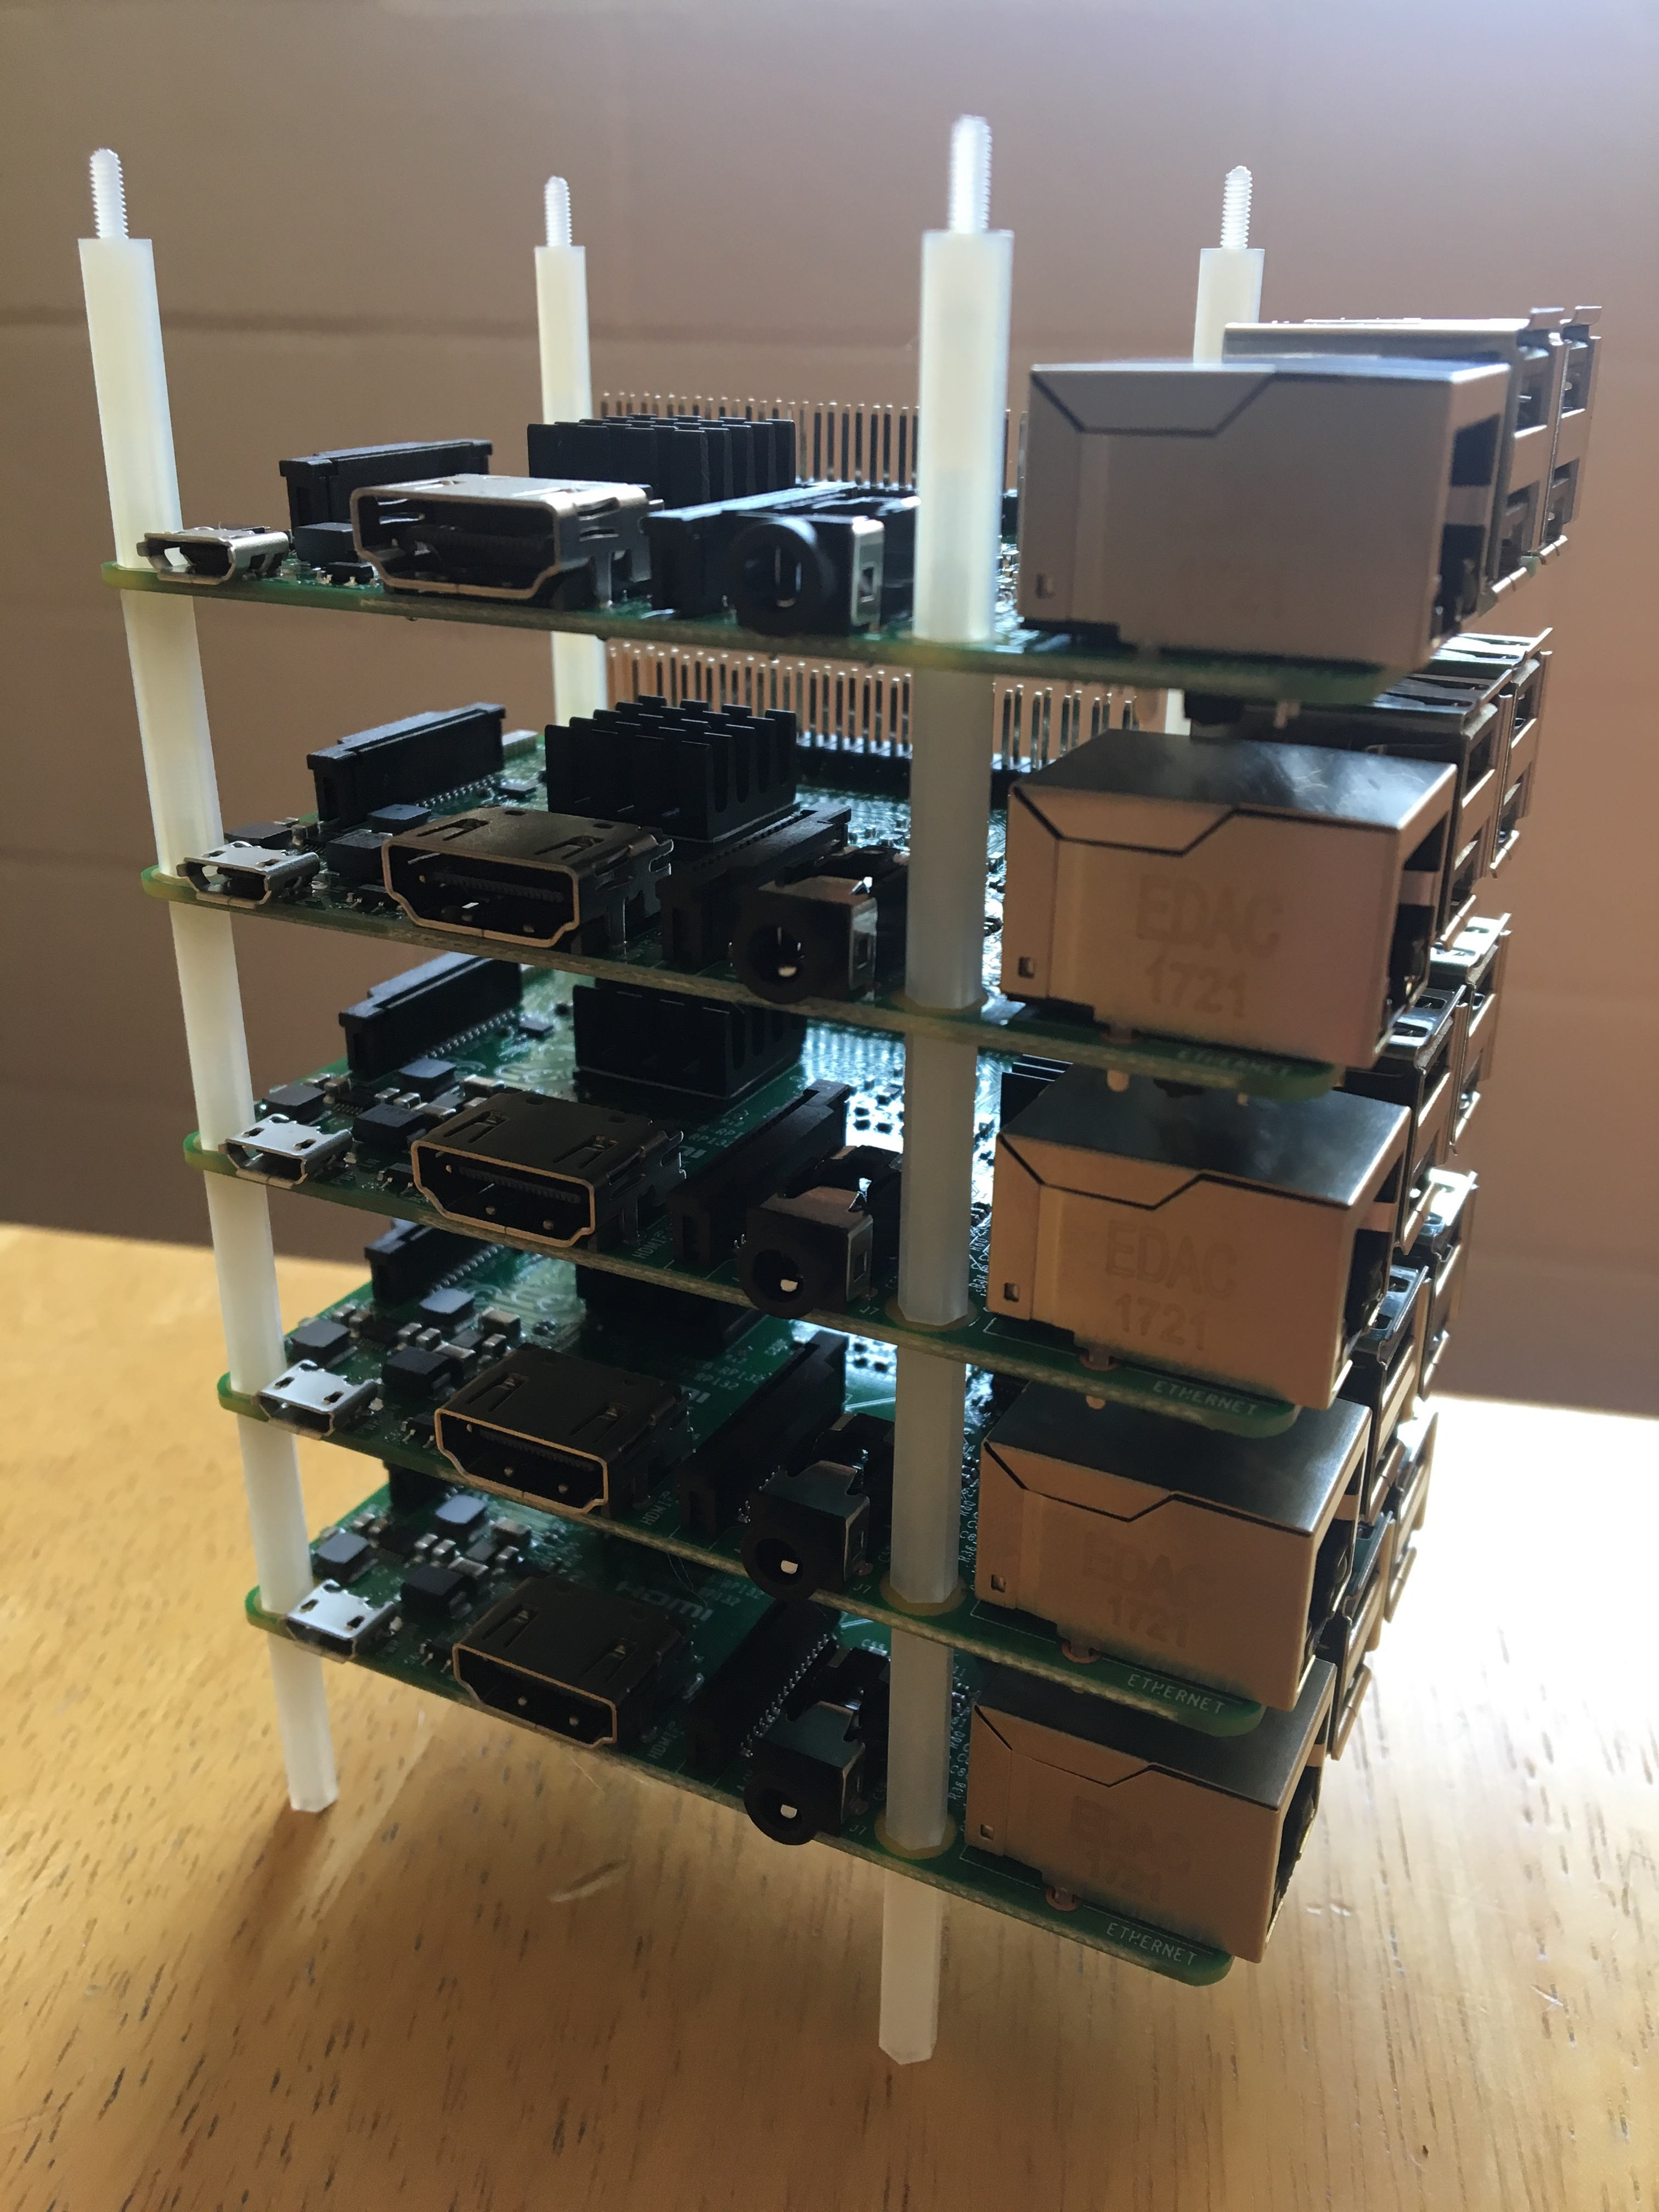
\includegraphics[width=\columnwidth]{images/pi-cluster-no-wires.jpg}
  \caption{5-node Pi cluster before wiring.}\label{f:cluster-no-wires}
\end{figure*}

Each node of the cluster is then attached to the switch using the ethernet cables. 

\section{Deployment}
\TODO{Finish Deployment section}
To configure the Raspberry Pis, first SD cards were burned using a
script that takes start and end machine id numbers as an input. The
option to perform DHCP setup can be enabled with a flag. If DHCP is
not used, the script assigns static IPs to each machine.

\section{Data}

The data used for the project is the Polarity Data 2.0, which is a dataset of 
movie reviews, first used by Bo Pang and Lillian 
Lee~\cite{hid-sp18-405-sentiment-pang2004asentimental}~\cite{hid-sp18-405-sentiment-pang2002thumbs}.
 The dataset includes 1000 positive and 1000 negative processed reviews, 
which are labelled with respect to their overall sentiment polarity. 

Each of the review is in a format of text file, and each of the single line in a 
file is corresponding to a sentence. Further, every token (which includes 
single word, punctuation marks, numbers) has been separated by space. For 
example, Figure~\ref{f:data} shows several lines in one of the movie reviews 
with line number on the right, which illustrate the two features mentioned 
above. These features play an important role in the sentiment analysis 
algorithm especially under map-reduce framework, which will be discussed in 
details in Section~\ref{s:algorithm}.
\begin{figure*}[!ht]
	\centering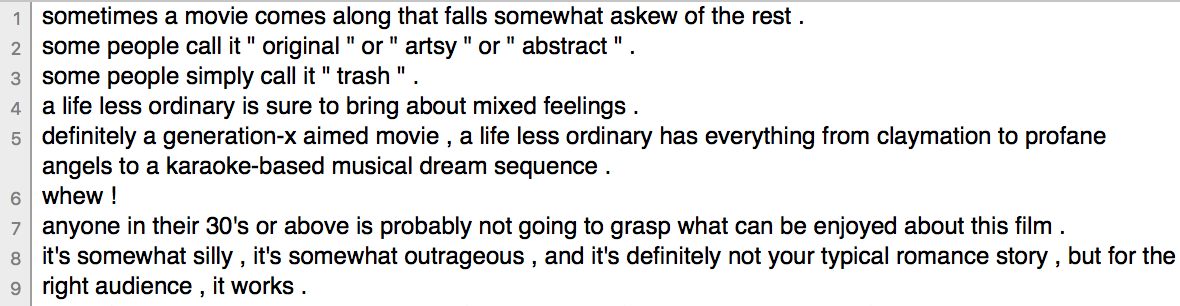
\includegraphics[width=\columnwidth]{images/polarity-data.png}
	\caption{Example Data File}
	\label{f:data}
\end{figure*}

The data is directly pulled from the 
source~\cite{hid-sp18-405-sentiment-data} and then split into training and 
testing sets according to a ratio of 8:2. The authors also keep the original 
ratio of positive and negative reviews in both the training and testing data 
sets. As a result, there are 1600 reviews (800 positive and 800 negative) in 
the training data set and 400 reviews (200 positive and 200 negative) in the 
testing data set. The splitting process is done by using the random sort 
functionality in bash with a fixed random seed to ensure consistency of 
performance benchmarking on different clusters. 


\section{Algorithm}
\label{s:algorithm}

\section{Benchmarking Process}
\TODO{Describe MapReduce task used for benchmarking.}


\section{Results}
\TODO{Add results.}

\begin{table}[hbt]
\centering
\caption{Benchmarking results}\label{t:results-table}
\begin{tabular}{llll}
Platform    & Docker & Deployment time & MapReduce Time \\
Pi 5 nodes  & Yes    & TBD             & TBD            \\
Pi 5 nodes  & No     & TBD             & TBD            \\
Echo        & Yes    & TBD             & TBD            \\
Echo        & No     & TBD             & TBD            \\
\end{tabular}
\end{table}



\section{Conclusion}

\TODO{Put here an conclusion. Conclusion and abstracts must not have any
citations in the section.}


\begin{acks}

  The authors would like to thank Dr.~Gregor~von~Laszewski for his
  support and suggestions to write this paper.

\end{acks}

\bibliographystyle{ACM-Reference-Format}
\bibliography{report}
